\makeatletter
\newcommand*{\textoverline}[1]{$\overline{\hbox{#1}}\m@th$}
\makeatother

\subsection{Levelshifters}\label{sec:levelshifter}
To generate sufficient output power thick-oxide transistors are used at the output stage. They can generate larger currents compared to thin oxide transistors and support a larger supply voltage. Thick-oxide transistors have the problem that their threshold voltage is too large to drive them with thin-oxide transistors. Also, the desired gate voltages for the thick-oxide PMOS transistors is entirely out of the DFE's output voltage range. Increasing the supply voltage of the thin-oxide transistors is not possible, since any supply voltage above 1.2V breaks them. Therefore a levelshifter is designed to drive the thick-oxide transistors. In this design special care is taken to ensure that the voltages across any thin-oxide transistor do not exceed 1.2V, so they do not break. On the output side the levelshifter has to be able to drive very large transistors. The driven NMOS transistors has to be supplied with a voltage of 0V(off) to 2V(on) and the driven PMOS transistors with a voltage of 5V(off) to 3V(on). 
In~\cite{powerdac} a design for the levelshifter was proposed, but they were not able to integrate it with the rest of their design. Some other designs that were looked at are proposed in~\cite{koo2005new} and~\cite{hass2000level}. In this paper the design from~\cite{powerdac} is chosen, because the others did not look as promising and are intended for different scenarios compared to the situation in this paper. Designing the levelshifter caused some major problems. First the cadence models originally used have have an unrealistically high threshold voltage of 1.5V, this makes it difficult to drive them with the thin oxide transistors. In order to create a functioning simulation this was changed to a more realistic threshold voltage of 0.7V. This gives a larger $V_{ON}$, making the transistors conduct more current for a smaller size. This is necessary, because the transistors being driven by the levelshifter are very large. Therefore a large driving current must be supplied by the levelshifter.
The levelshifter design started with the design of the PMOS driver, which should have an output voltage of 3(off) to 5V(on). As a starting point the design from~\cite{powerdac} was used, it is shown on the right in Fig.~\ref{fig:schematic_levelshifter}. In this design the thick oxide transistors M3 and M4 serve to protect the thin oxide transistors M5 and M6 from too high voltages. M1 and M2 form a current sensing circuit that charge the output node and each other's gates when switching. Their most important parameter is their width, the larger they are the quicker they charge the output. But a larger M1 and M2 also means that the M3-6 need to be larger to discharges the nodes. Since M2 must drive both M1 and the load it must be bigger than M1. The next most important parameters are the lengths of M3 and M4 and widths of M5 and M6. Together they determine the speed at which the output nodes are discharged and the voltage level of the output nodes when M3 and M5 or M4 and M6 are active. The circuit operates as follows. Assume initially VIN is high and \textoverline{VIN} is low. Node \textoverline{VOUT} will be pulled low by the left branch and the right branch will not conduct any current. Then \textoverline{VOUT} is pulled towards 3V and M2 will start conducting and charging node VOUT towards 5V. This will make M1 stop conducting current, causing \textoverline{VOUT} to be pulled even closer to 3V. In this way M2 and M1 drive each other's gate and amplify each other, enabling fast switching. When everything is settled VOUT should be near 5V and \textoverline{VOUT} near 3V. When the input switches (VIN goes low and \textoverline{VIN} goes high) the process is reversed. Node VOUT will be pulled towards 3V and no current will be conducted by the left branch, enabling \textoverline{VOUT} to be driven towards 5V. Again, M1 and M2 will amplify this process and switch VOUT from 5V to 3V and vice versa for \textoverline{VOUT}.
To drive the NMOS transistors of the DAC's output current sources an extra stage is added to the levelshifter. Because the threshold voltage is lowered to 0.7V the VIN signal can drive M8 to pull the output to 0V when VIN is high. However this is not ideal since VIN does not create a large $V_{ON}$. VOUT is high then, so M7 will not conduct current. When VIN is low, VOUT is near 3V and M7 will conduct current, pulling VOUT\_NMOS to 2V. For the NMOS driver important parameters were the length of M7, which largely determines the maximum voltage of the output, and the widths of both M7 and M8, which mostly detemine the speed at which it can switch the load. For both the PMOS and NMOS drivers VBIAS determines the maximum $V_{DS_{5,6}}$ and is set to make sure $V_{DS_{5,6}}$ has a maximum value of 1.2V.
\begin{figure}[h]
 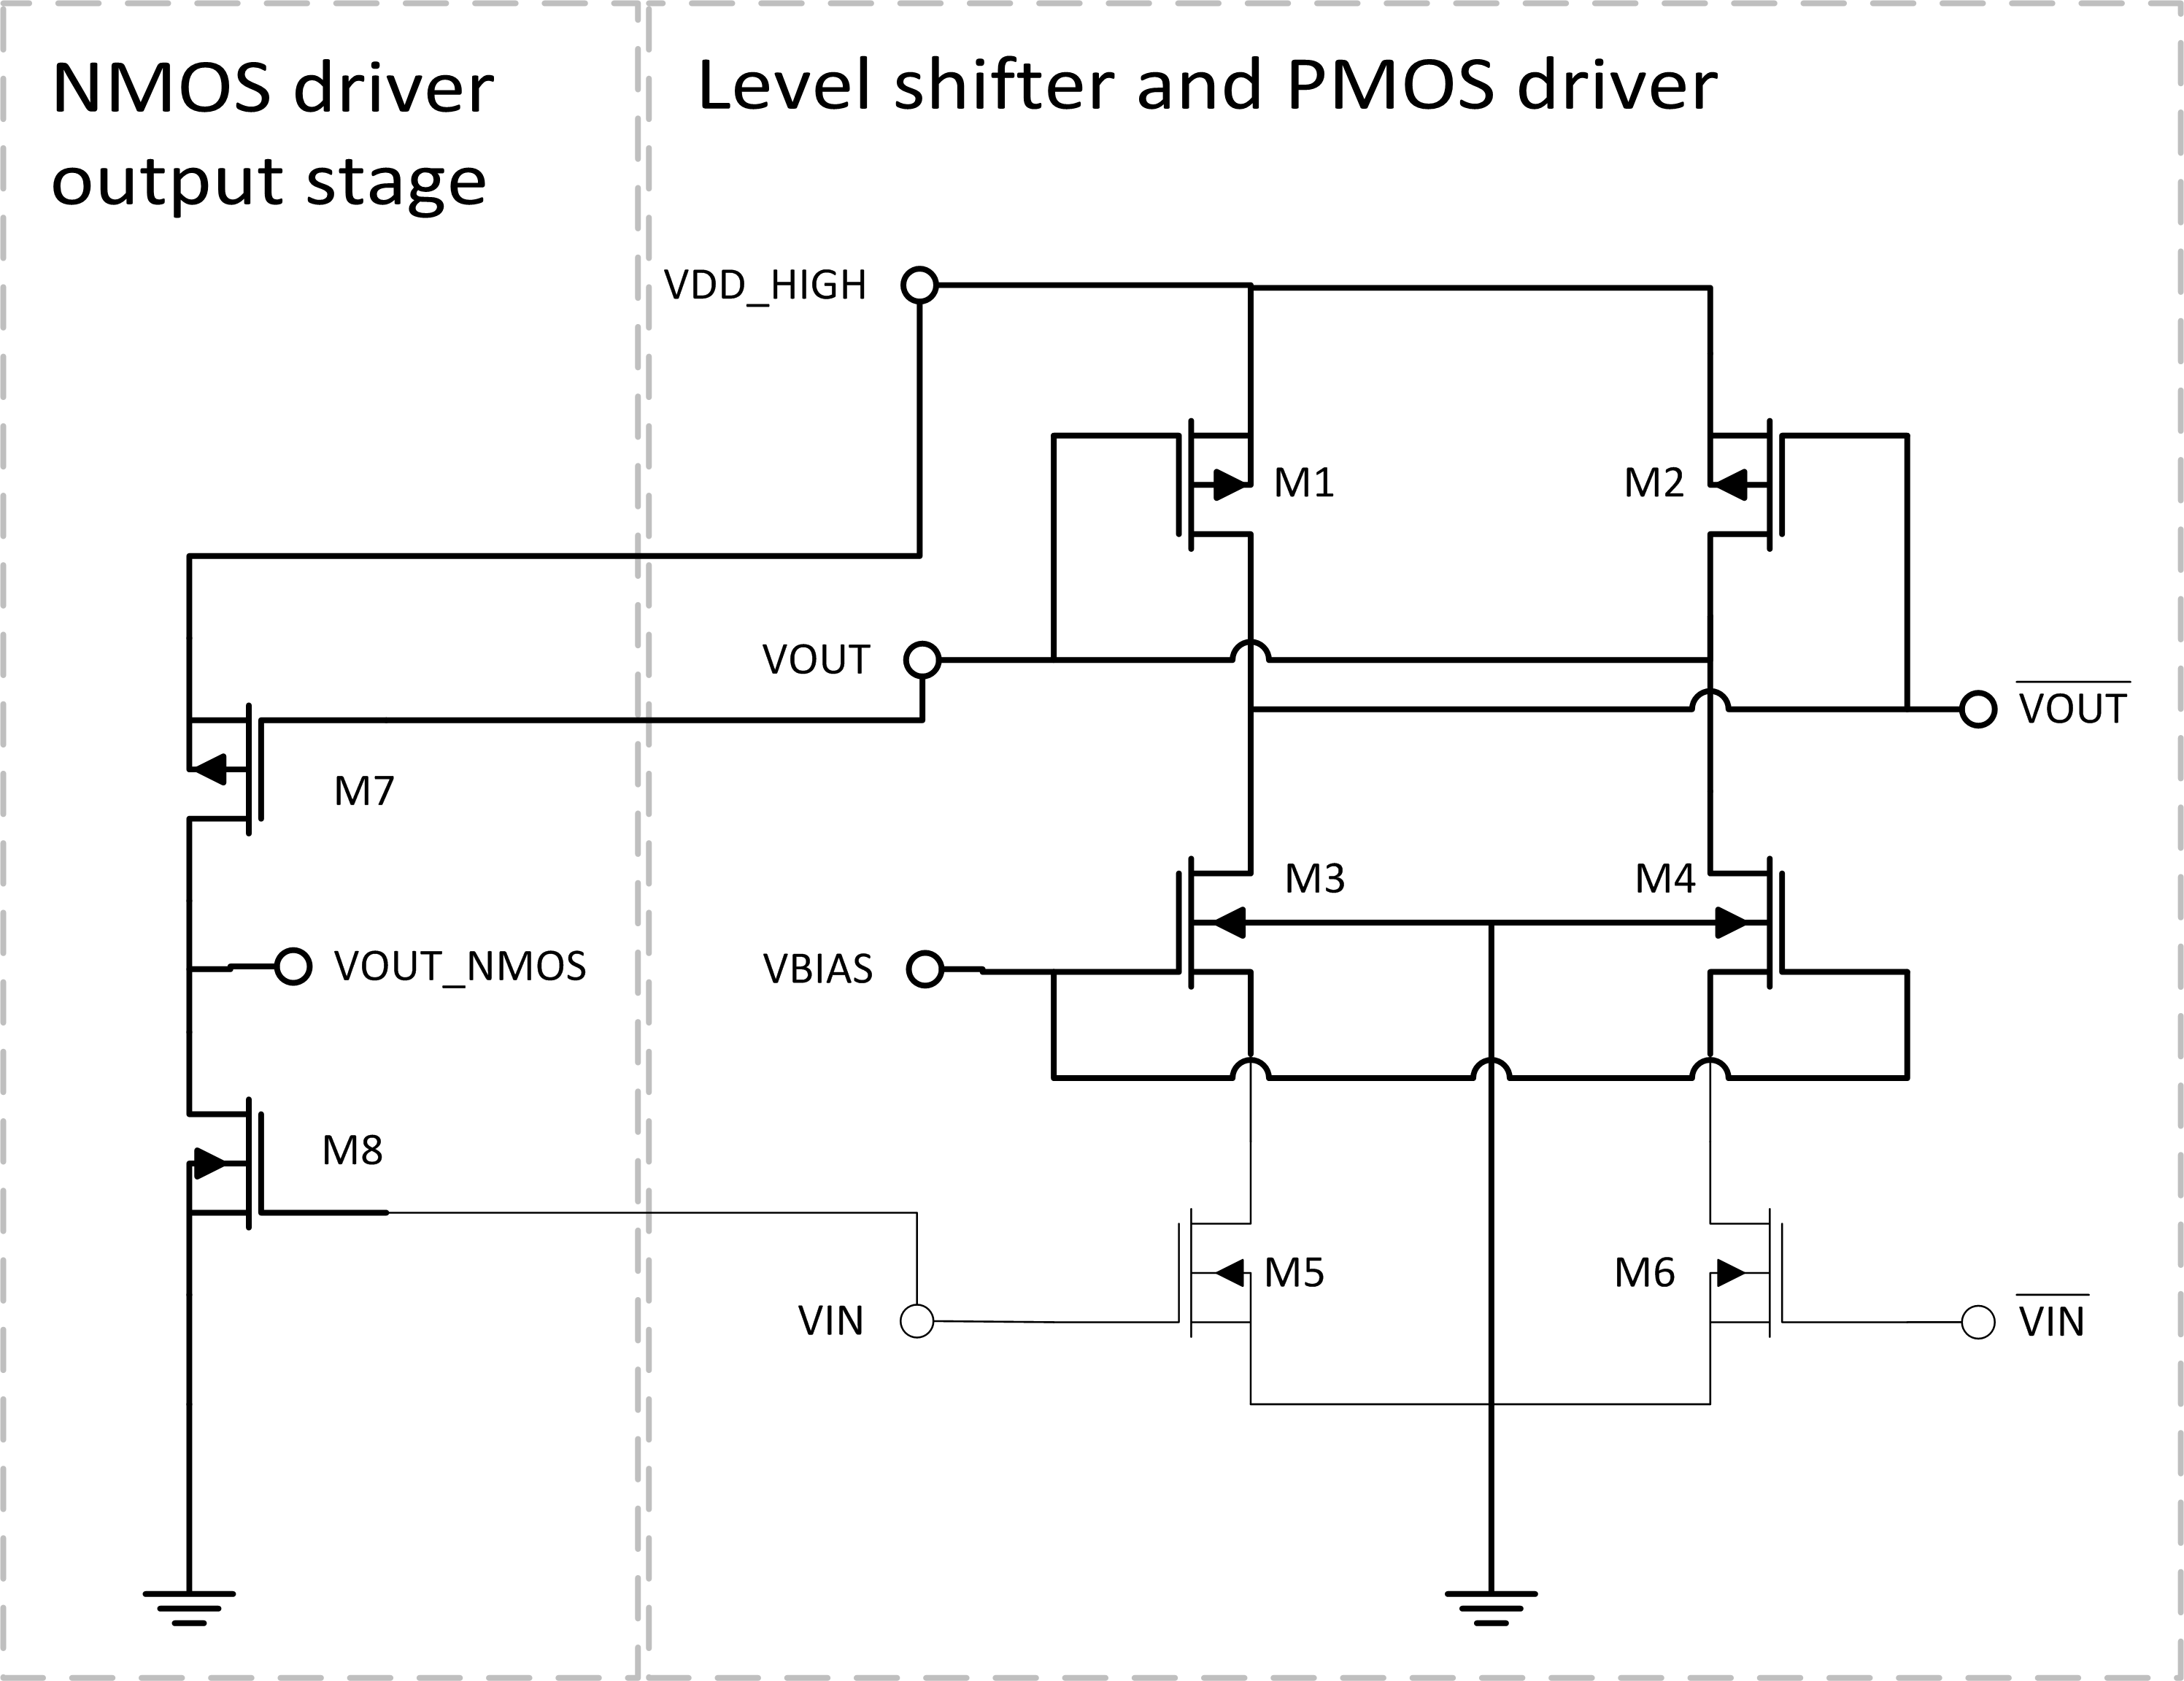
\includegraphics[width=0.5\textwidth]{levelshifter_schematic}
 \caption{Schematics of the levelshifter, thick wires indicate a high voltage regime and thin lines the low voltage transistors. On the right the up-shifting PMOS driver is shown. Its output VOUT can drive a PMOS transistor. The NMOS driver's layout is the same with an extra stage added on the left side. The node VOUT\_NMOS can drive a NMOS transistor.}
 \label{fig:schematic_levelshifter}
\end{figure}
The final sizes of transistors in the PMOS and NMOS driving levelshifters are listed in Appendix~\ref{sec:appendix} in Tables~\ref{Tab:Levelshifter_PMOS_sizes} and~\ref{Tab:Levelshifter_NMOS_sizes} respectively. How these sizes have been determines is discussed next. Both M1 and M2 should have a $V_{DS}$ as low as possible, so their length is set to the minimum of 200n. Their widths determines how fast they can charge the load and each other and were determined using a sweep over both the widths and choosing the best result. Other important parameters are the lengths of M3 and M4, widths of M5 and M6 and $V_{BIAS}$. These have been determined by sweeping over all three parameters and choosing the best options. The result of this simulation is shown in Fig.~\ref{fig:levelshifter_sweep_PMOS}. The configuration with the steepest edges that comes closest to 3V, to keep the load PMOS in saturation, has been chosen. Finally the other parameters are finetuned.
\begin{figure}[h]
 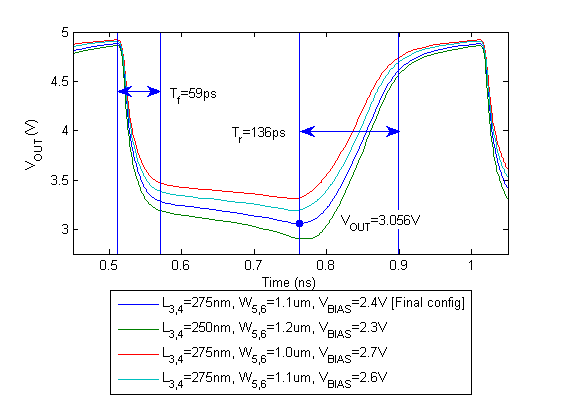
\includegraphics[width=0.5\textwidth]{Levelshifter_sw_ln34_wn56_vbo.png}
 \caption{Parameter sweep over the of the lengths of M3 and 4, widths of M5 and 6 and $V_{BIAS}$. For clarity only a selection and the chosen configuration are shown. The load is a thick oxide PMOS transistor of 200nm by 60$\mu$m.}
 \label{fig:levelshifter_sweep_PMOS}
\end{figure}
To determine the sizes of the transistors of the NMOS driver the PMOS driver is used a starting point. This works since the original circuit still only drives one PMOS transistor. So initial tuning of M7 and M8 will have little effect on the behaviour of the original circuit. The maximum output voltage level is determined mostly by the dimensions of M7. The dimensions of M8 determine how fast the output voltage drops. Because the off voltage must be as close to 0V as possible, the length of M8 is set to the minimum of 200nm. Its width and the dimensions of M7 are chosen using a combined sweep. A selection of some resulting characteristic curves are shown in Fig.~\ref{fig:levelshifter_sweep_NMOS}. The output voltage is mostly determined by $L_7$. The ratio between $W_7$ and $W_8$ largely determines the output characteristic. The chosen parameters are $L_7=1.4\mu m, W_7=20\mu m$ and $W_8=25\mu m$.
\begin{figure}[h]
 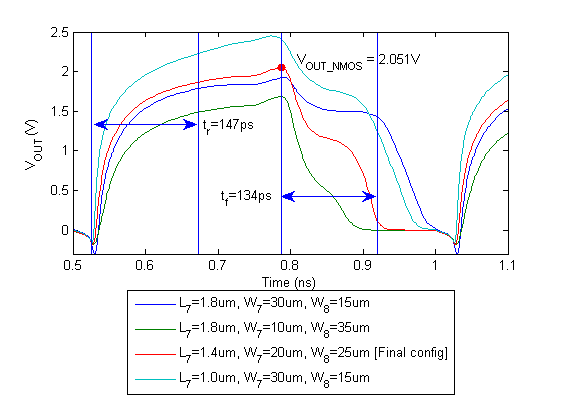
\includegraphics[width=0.5\textwidth]{Levelshifter_sw_lp16_wp16_wn10.png}
 \caption{Parameter sweep over the of the length of M7 and widths of M7 and 8. For clarity only a selection with characteristic curves and the chosen configuration are shown. The load is a thick oxide NMOS transistor of 300nm by 12$\mu$m.}
 \label{fig:levelshifter_sweep_NMOS}
\end{figure}

%A final aspect of interest is the power consumption of the levelshifter. This is determined mostly by the current necessary for driving the load transistor. The %gates of the load are both charged and discharged via the levelshifter, causing most of the powerconsumption. But also the levelshifter's transistors are %relatively large and cost significant power to switch. Simulation results are not available yet. 